% Data and Empirical Analysis: Data
\subsection{Data}
\label{C3-SubSection:Data}
This section summarizes data on wells, geology, and oil prices, which are utilized to conduct empirical analysis and estimate a model of drilling behaviors observed in North Dakota. 

\subsubsection{Well Data}
\label{C3-SubSubSection:Well-Data}
Data for wells in North Dakota's Bakken region come from the Oil and Gas Division of the North Dakota Industrial Commission (NDIC), the regulator for the drilling and production of oil and gas in North Dakota.\footnote{NDIC's well data are available at \href{https://www.dmr.nd.gov/oilgas}{Official Portal for North Dakota State Government}.} NDIC-providing well data include a complete index of all wells permitted in North Dakota. The data contains basic information for each well, such as the type of well, completion and spud dates, location, the first and the current operator names, and targeting pool. Individual well's projection and injection histories, including producing days during each month, are also contained in the data. 

Detailed well completion data are also obtained from NDIC.\footnote{Using Form 6, Well Completion or Recompletion Report, filed by operators, NDIC has developed the detailed data.} The data contain how much water and proppant were consumed during well simulations.

The regulatory body also provides well-level survey data. The survey data include directions and lengths of legs in a well. Using the leg-related information in the data, we compute the total length of horizontal drillings in an individual well. 

The sample used throughout this paper consists of 24,520 horizontal wells that targeted the Bakken pool.\footnote{The Bakken pool includes Bakken, Three Forks, and Sanish formations.} Summary statistics for those wells are presented in Table \ref{Table:Summary-Statistics-for-Horizontal-Wells}.


\subsubsection{Geological Survey Data}
\label{C3-SubSubSection:Geological-Survey-Data}
We obtain geological survey data from the North Dakota Geological Survey (NDGS).\footnote{To be specific, we exploit NDGS maps GI-59 and GI-63.}  Regarding the upper and the lower Bakken shales, their estimates of thickness, thermal maturity, and total organic contents are illustrated in the geospatial data. We follow \cite{Experiential-and-Social-Learning-in-Firms_Covert_2015} to match the three geological characteristics with each horizontal well in our sample.\footnote{Refer to Section 2.4.1 of \cite{Experiential-and-Social-Learning-in-Firms_Covert_2015}.} Figure \ref{Figure:Spatial-Distributions-of-Geological-Characteristics} demonstrates the spatial distribution of well-level geological features. 


\subsubsection{Oil Price Data}
\label{C3_SubSubSection:Oil-Price-Data}
\afterpage{
     \begin{figure}[t!]
         \centering
         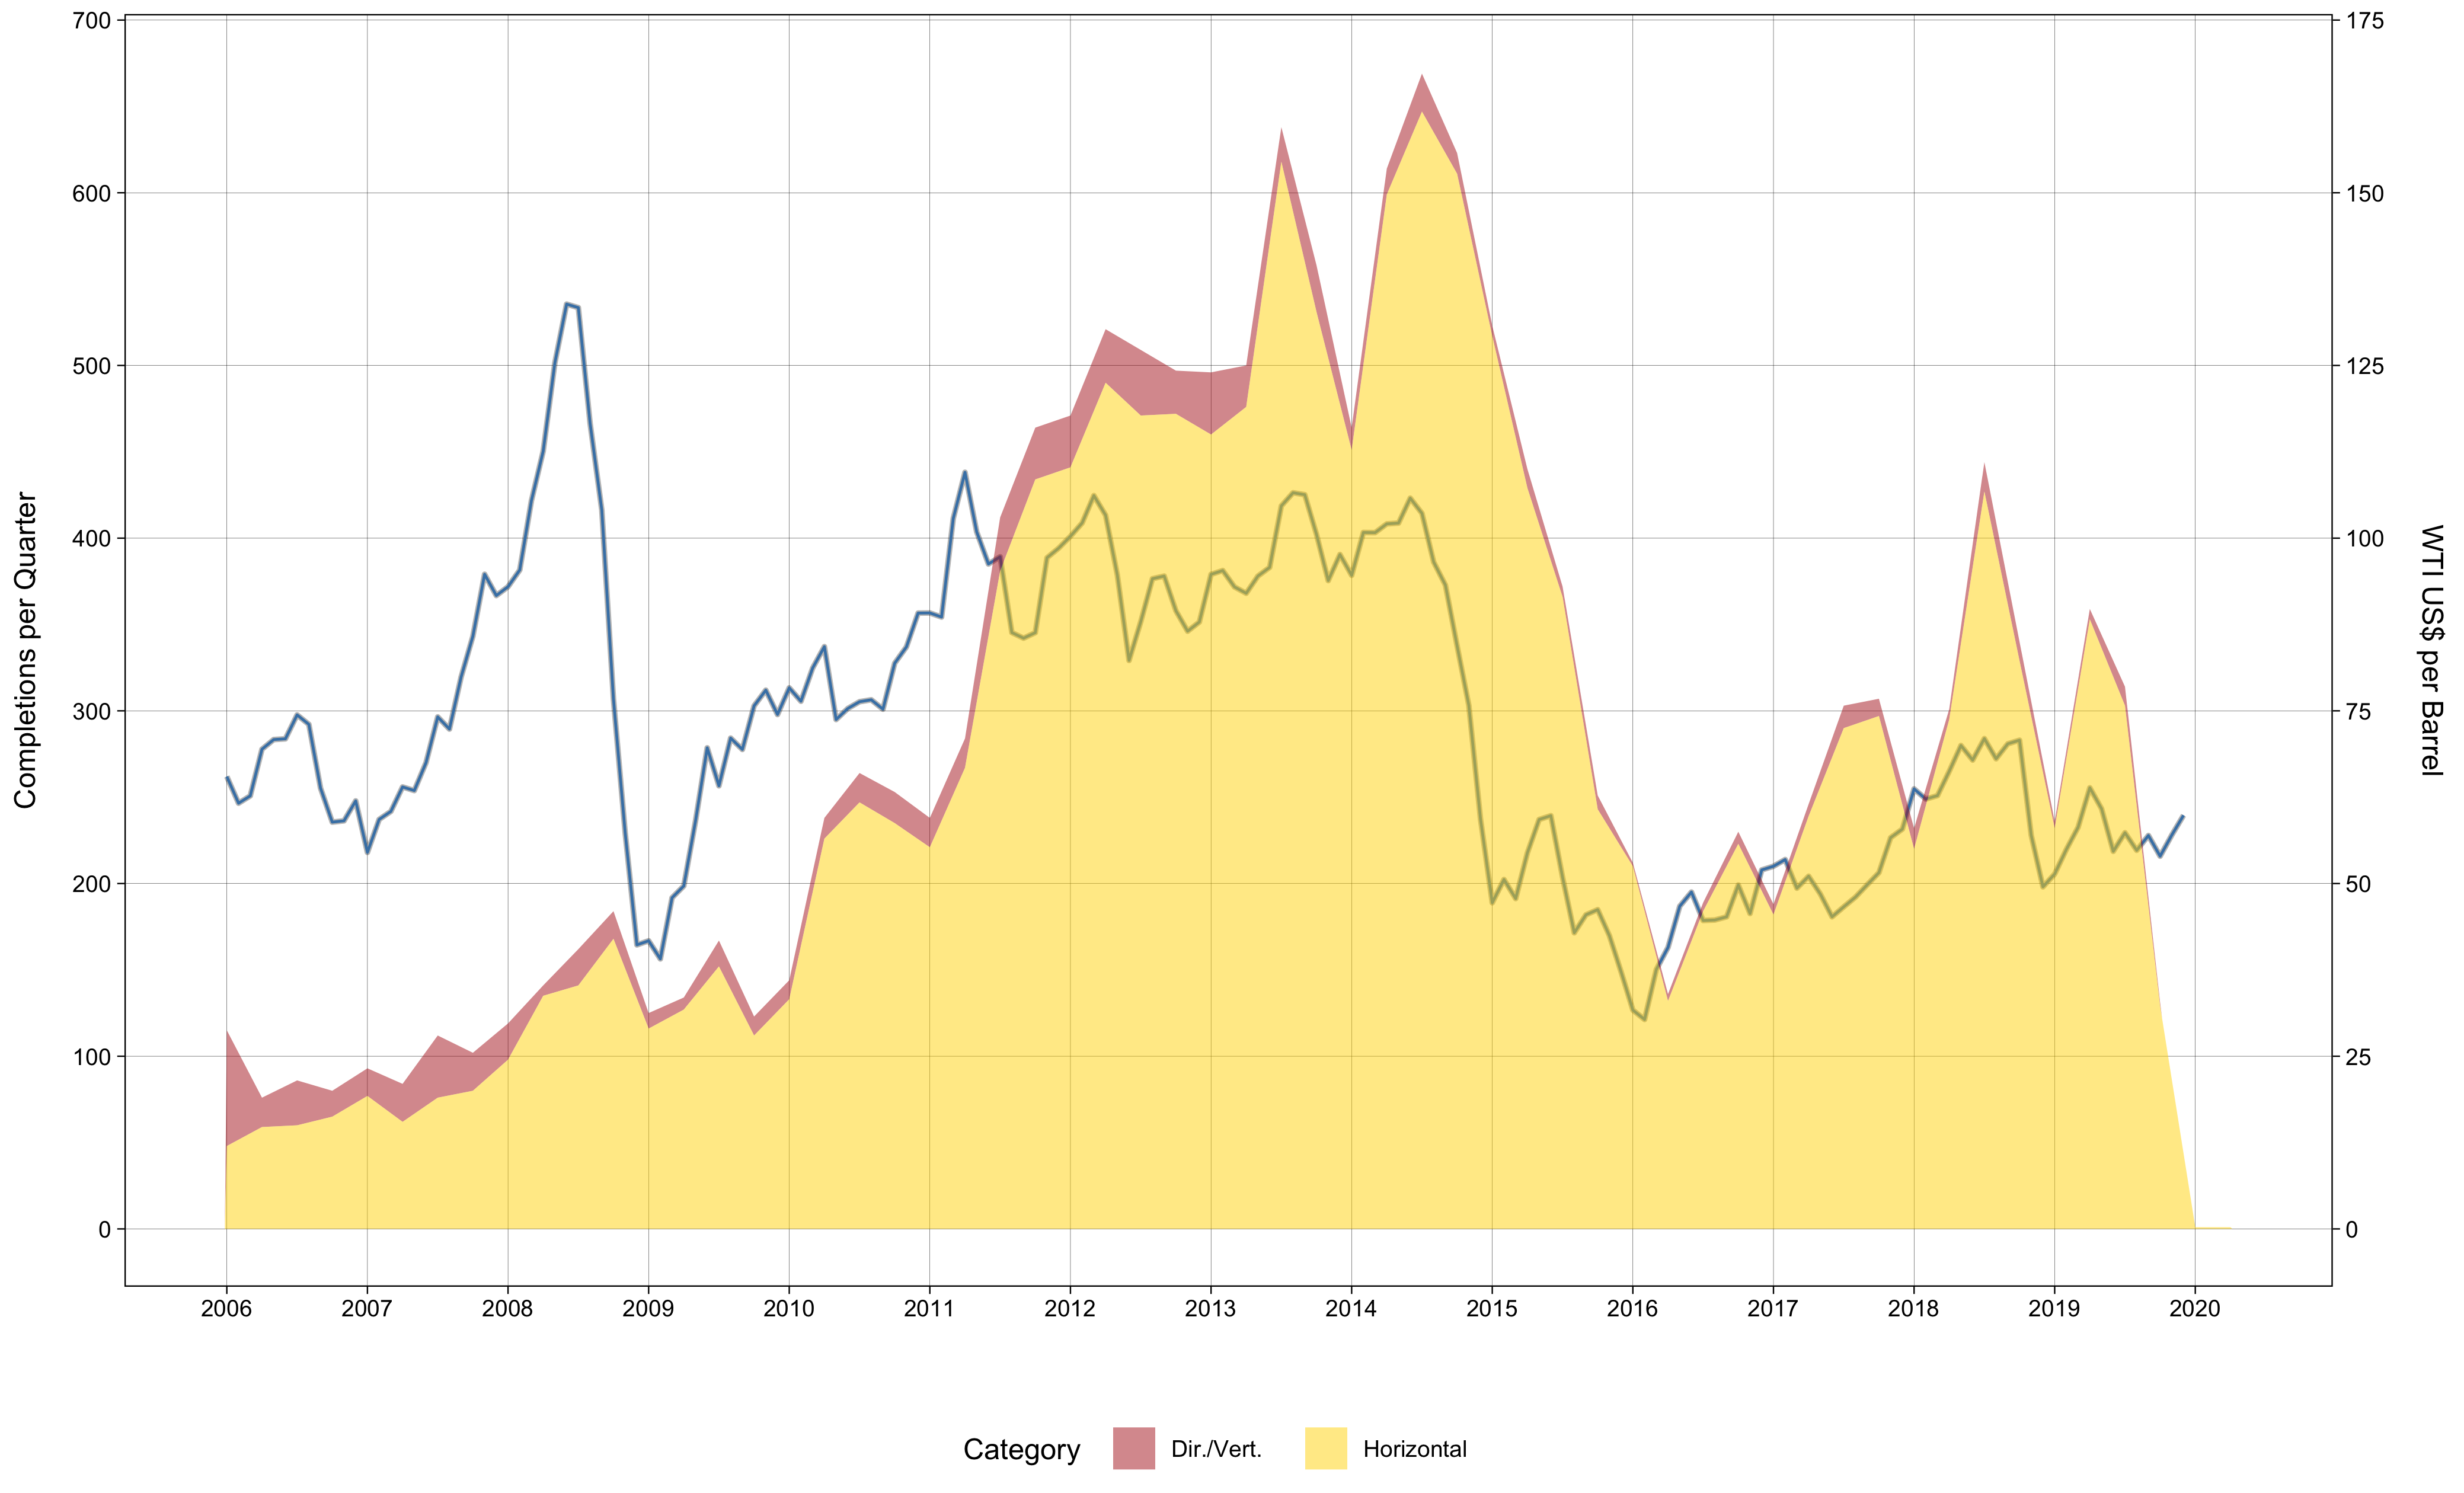
\includegraphics[scale = 0.105]{04_Chapter-3/00A_Figures/Figure_Completion-over-Time.png}
         \caption{Time Series of the Number of Well Completions in North Dakota}
         \caption*{
            {\small
             \textit{Note}: 
             This figure shows the time series of the number of well completions in North Dakota. Horizontal wells have been strictly dominant in that area. The solid line in the figure is the monthly per-barrel spot prices for West Texas Intermediate at Cushing, Oklahoma. The figure suggests that the spot prices positively correlate with horizontal well completions in North Dakota. 
         }}
         \label{Figure:Time-Series-of-the-Number-of-Well-Completions-in-North-Dakota}
     \end{figure}
}
We collect the monthly per-barrel spot prices for West Texas Intermediate at the Cushing, Oklahoma from the Energy Information Administration.\footnote{Time series data for Cushing, OK WTI Spot Price FOB is available \href{https://www.eia.gov/dnav/pet/PET\_PRI\_SPT\_S1\_M.htm}{here}.} As shown in Figure \ref{Figure:Time-Series-of-the-Number-of-Well-Completions-in-North-Dakota}, there was a striking movement in oil prices between 2014 and 2016. Specifically, oil prices, maintained at around \$100 per bbl during the first half of 2014, had continued to plunge, reaching less than \$50 per bbl in January 2015. After recovering to \$60 per bbl during the first half of 2015, oil prices had fallen to \$30 per bbl by the end of the year. Since then, oil prices have gradually risen until they declined again during the final quarter of 2018.



% Data and Empirical Analysis: Empirical Analysis
\subsection{Empirical Analysis}
\label{C3-SubSection:Empirical-Analysis}

\subsubsection{Correlation between Oil Prices and Horizontal Drilling in North Dakota}
\label{C3-SubSubSection:Correlation-between-Oil-Prices-and-Horizontal-Drilling-in-ND}
Figure \ref{Figure:Time-Series-of-the-Number-of-Well-Completions-in-North-Dakota} shows how well completions in North Dakota evolved between 2009 and 2020. As clearly illustrated, well completions, which were driven mainly by horizontal wells, dramatically increased from the beginning of 2010. 

According to the figure, it is evident that drilling horizontal wells in North Dakota is closely correlated with oil prices, especially after 2009. On the whole, oil prices significantly increased between 2009 and 2010 and remained high until mid-2014. And there was a sharp plunge in oil prices from mid-2014 to the end of 2015. The number of horizontal wells drilled in that time range significantly declined too. And when oil prices gradually climbed between 2016 and 2020, North Dakota's drilling activities also recovered. To summarize, oil prices and the number of horizontal drilling in North Dakota seem to be positively correlated. Importantly, such a positive correlation between oil prices and horizontal drilling in the state suggests that fracking firms' drilling decisions strongly depend on oil prices. In Section \ref{C3-SubSubSection:The-Role-of-Geological-Quality-in-Horizontal-Drilling}, we show that their drilling decisions are linked with oil prices through the geological features of well sites.


\subsubsection{The Role of Geological Quality in Horizontal Drilling}
\label{C3-SubSubSection:The-Role-of-Geological-Quality-in-Horizontal-Drilling}
\textit{\textbf{Estimation of Unobservable Geological Characteristics of Horizontal Wells}} --- Not all well-specific information on geological features is available to econometricians. The NDGS geological survey data only include estimates of four different measurements of geological properties at a given location. Because the geospatial data was published to the public in 2008, it is likely that fracking firms, whose objective is to maximize their profits, have already exploited the contents of the maps. As discussed in \cite{Learning-where-to-drill_Agerton_2020}, learning about the spatial distribution of deposits by drilling wells is one of three economic factors that govern firms' where-to-drill decisions. So, it is reasonable to suppose that firms have private information about the Bakken area's spatial distribution of geological characteristics, which is not accessible to researchers. 

The geological characteristics observed only by firms play two different roles in their drilling decisions. First, firms choose whether to drill a location based on its resource quality. Thus, the sample of wells we observe is not random: it has been selected based on unobservable (to us) resource quality. Second, firms' choice of inputs during hydraulic fracturing of each well may be correlated with the unobservable resource quality. For these reasons, accounting for resource quality is critical in modeling firms' decisions and production functions. 

Following \cite{The-Economics-of-Time-Limited-Development-Options_2020_Herrnstadt-Kellogg-and-Lewis}, we employ Robinson's partially linear model to determine the unobservable quality of the horizontal wells completed between 2009 and 2018. We first specify the oil production from a horizontal well as
\begin{equation}
\begin{split}
    \log \left( y_{i} \right) \ 
    & = \ \log \left( \boldsymbol{X}_{i} \right)' \boldsymbol{\beta} \ - \ \lambda \left( longitude_{i}, latitude_{i} \right) \ + \ \epsilon_{i}.
\end{split}
\label{Equation:Production-Function}
\end{equation}
In this specification, $y_{i}$ are horizontal well $i$'s cumulative oil production at its cumulative production month 24.\footnote{That is, unobservable geological features are estimated cross-sectionally in our estimation.} The covariate vector $\boldsymbol{X}_{i}$ for well $i$ includes hydraulic fracturing inputs (i.e., fluid volume, proppant weight, and length of horizontal drilling), cumulative producing days, and observable geological characteristics (i.e., thickness, total organic contents, and thermal maturity). The term $\lambda(longitude_{i}, latitude_{i})$ is a nonparametric function of each well's coordinates and captures well $i$'s unobservable resource quality. Lastly, $\epsilon_{i}$ is a productivity shock not correlated with resource quality. 

To operationalize model (\ref{Equation:Production-Function}), we estimate the following partially linear model:
\begin{equation}
\begin{split}
    \log \left( y_{i} \right) \ - \ \widehat{m}_{y_{i}} \ 
    & = \ \left( \log \left( \boldsymbol{X}_{i} \right) \ - \ \widehat{\boldsymbol{m}}_{\boldsymbol{X}_{i}} \right)' \boldsymbol{\beta} \ + \ \epsilon_{i}.
\end{split}
\label{Equation:Partially-Linear-Model}
\end{equation}
Here, $\widehat{m}_{y_{i}}$ are predictions from a non-parametric regression of $\log \left( y_{i} \right)$ on well $i$'s coordinates $(longitude_{i}, latitude_{i})$. The $\widehat{m}_{y_{i}}$ terms are smoothed means. Differencing these means out serves the same role as the within-transformation in a fixed effects model. In fact, if one used a uniform kernel function, $\widehat{m}_{y_{i}}$, within discrete cells, the estimator would be mathematically identical to fixed effect estimation with spatial fixed effects for each well. Predictions $\widehat{\boldsymbol{m}}_{\boldsymbol{X}_{i}}$ are obtained from different nonparametric regressions whose dependent and independent variables are $\log \left( \boldsymbol{X}_{i} \right)$ and $(longitude_{i}, latitude_{i})$, respectively. The values of primary interest $\widehat{\lambda}_{i}$ (i.e., the unobservable geological quality of horizontal well $i$) are estimated as follows\footnote{For details of Robinson's difference estimator, refer to \textit{9.7.3 Partially Linear Model} in \cite{MicroEconometrics-Methods-and-Applications_Cameron-and-Trivedi_2005}.}:
\begin{equation}
\begin{split}
    \widehat{\lambda}_{i} \
    & = \ \widehat{m}_{y_{i}} \ - \ \widehat{\boldsymbol{m}}_{\boldsymbol{X}_{i}}' \widehat{\boldsymbol{\beta}}
\end{split}
\label{Equation:Estimates}
\end{equation}
\afterpage{
    \begin{figure}[t!]
        \centering
        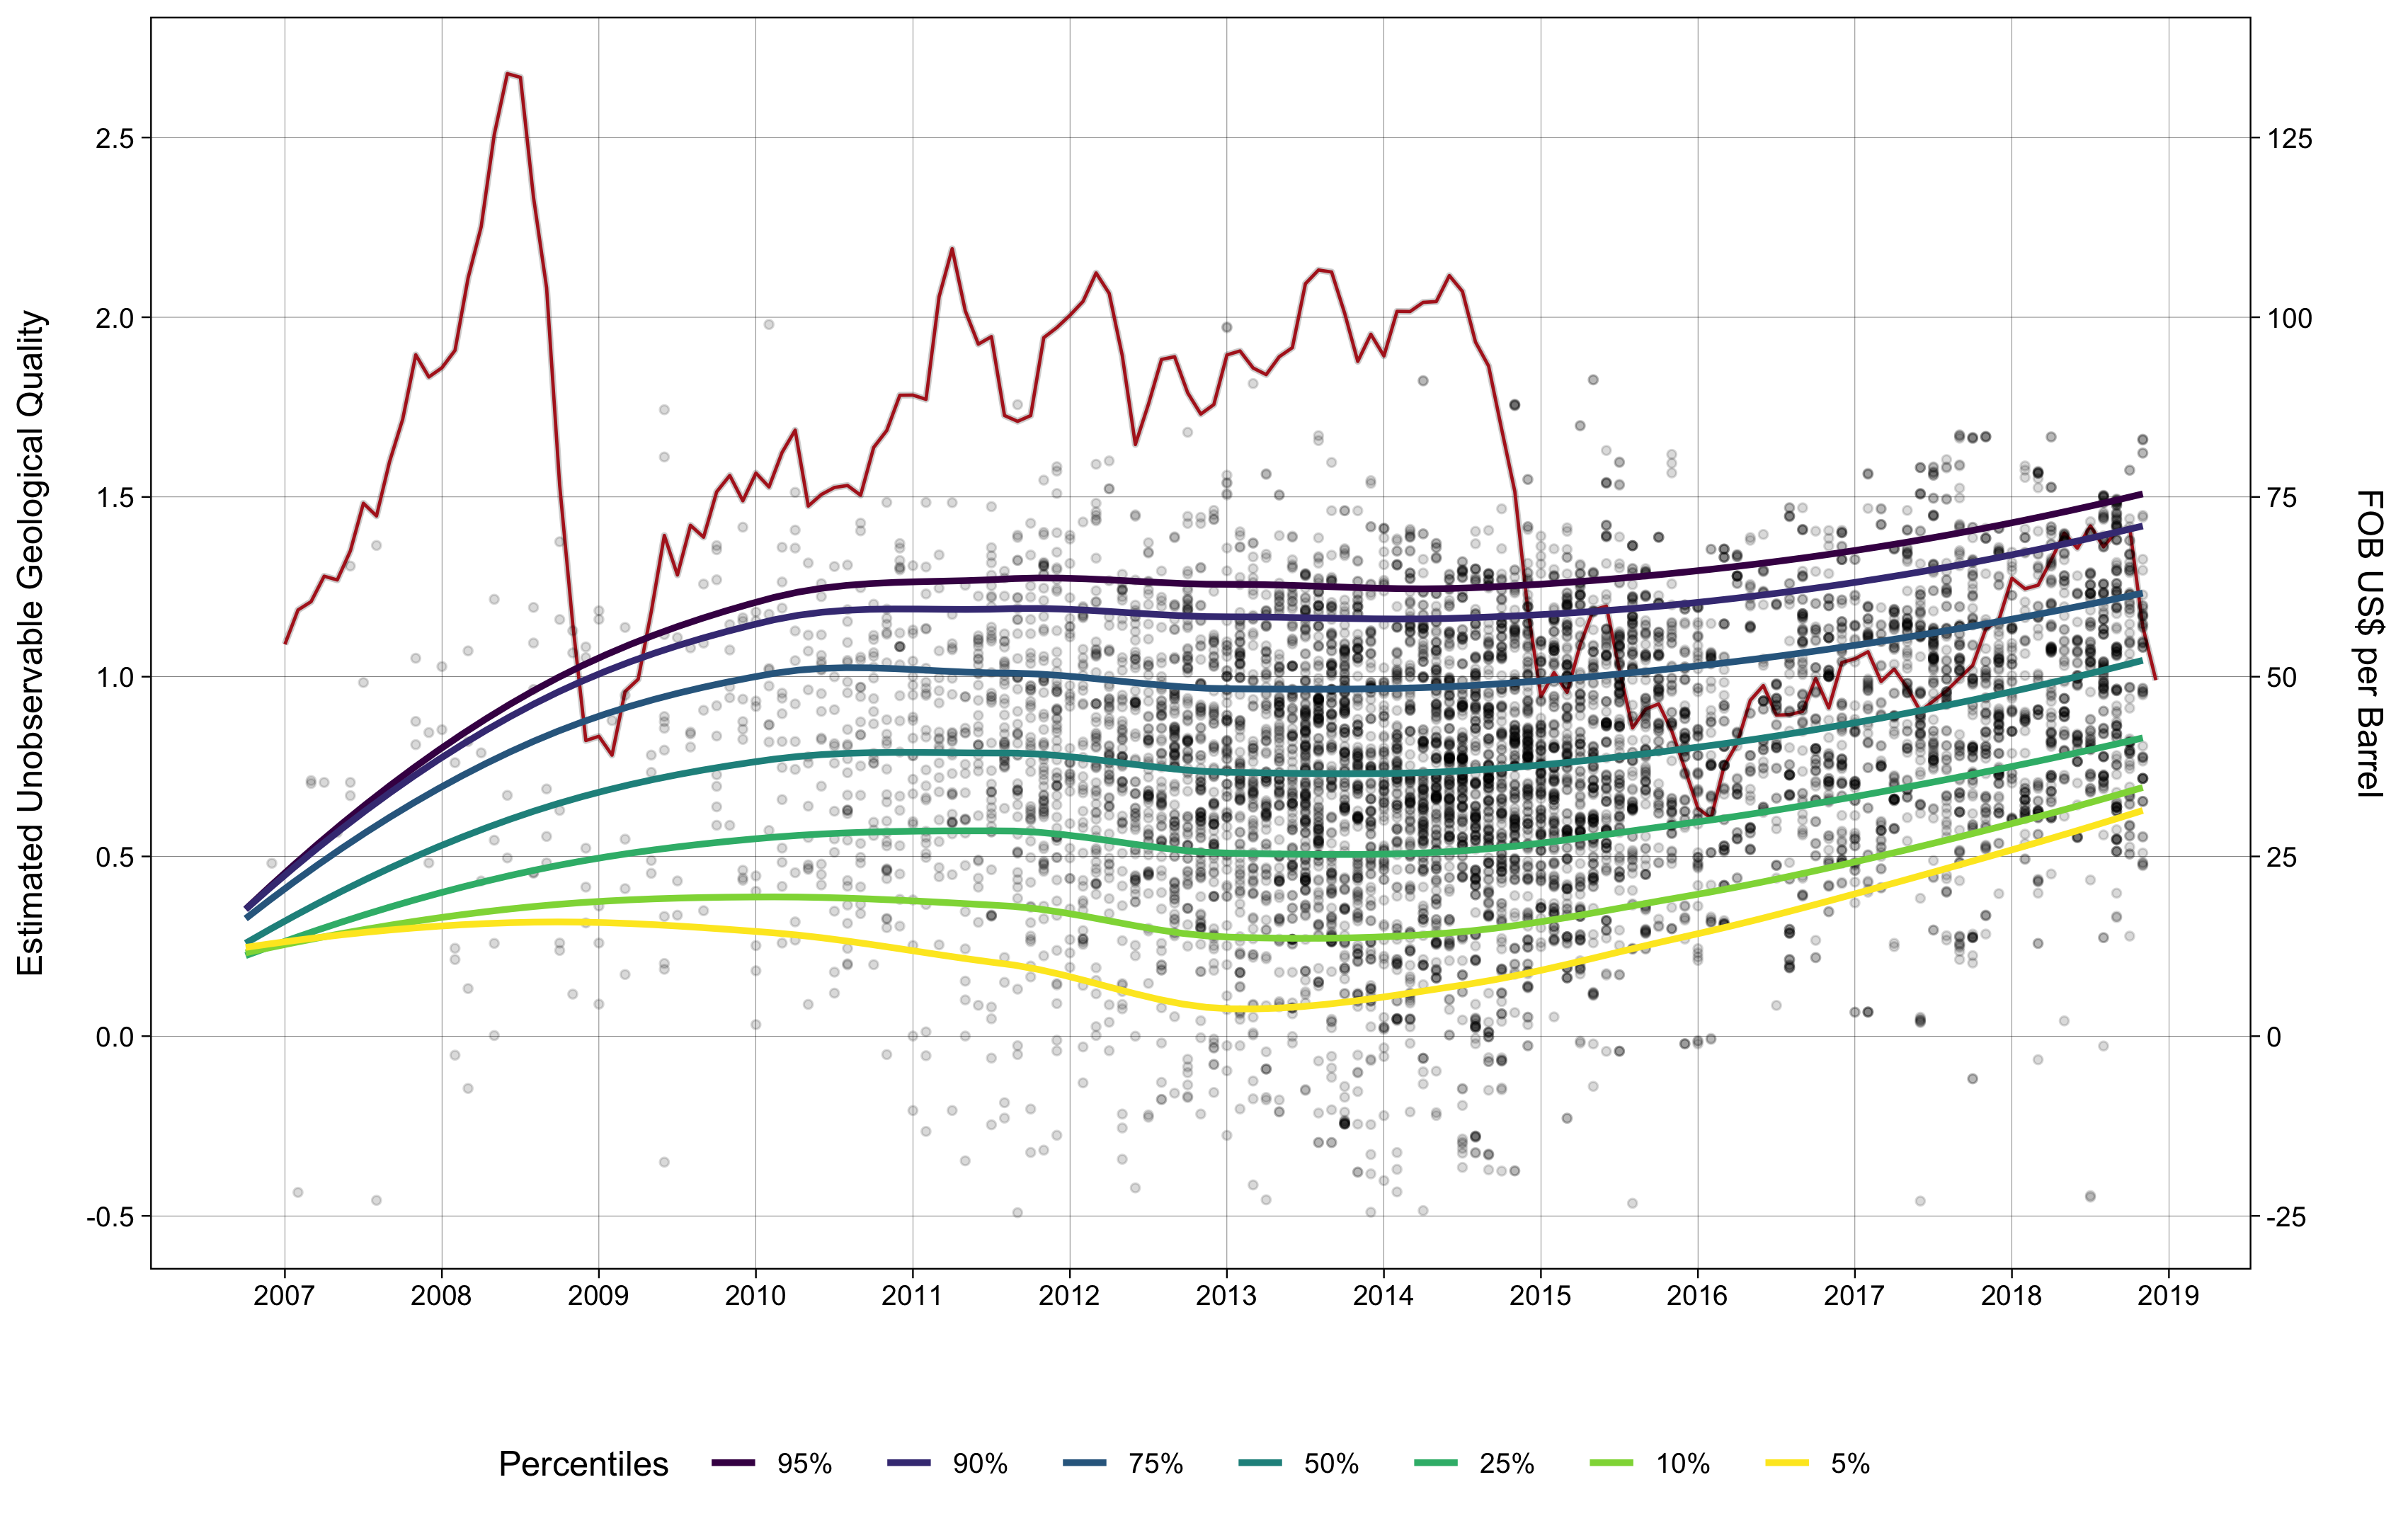
\includegraphics[scale = 0.13]{04_Chapter-3/00A_Figures/Figure_Cross-Sectional-Approach_Estimates-from-Robinson-Estimator_Time-Trend-of-Unobservable-Geological-Quality.png}
        \caption{Simultaneous Drilling of Horizontal Wells with Heterogeneous Geological Quality}
        \caption*{
            {\small
            \textit{Note}: 
            This figure indicates the estimated geological feature for each horizontal well, depicted as a dot. Those dots definitely suggest the simultaneous drilling of horizontal wells with heterogeneous geological quality. In the figure, percentiles of the estimates, with the 95\% confidence interval of each, are also presented. The solid red line is the time series of the monthly per-barrel spot prices for West Texas Intermediate at Cushing, Oklahoma. Oil prices plunged significantly between 2014 and 2015 and rose gradually. The percentile lines skewed upward, especially lower ones, as of the second half of 2014.  
        }}
        \label{Figure:Simultaneous-Drilling-of-Horizontal-Wells-with-Heterogeneous-Geological-Quality}
    \end{figure}
}
In our analysis, we define low- and high-quality locations by dividing our sample of well sites into those with $\widehat{m}_{y_{i}}$ below and above the median. Even though $\widehat{m}_{y_{i}}$ is estimated from only higher-quality locations with observed drilling, and therefore biased upward, the ordinal ranking of well sites should be affected less. Figure \ref{Figure:Spatial-Distribution-of-the-Estimated-Geological-Characteristic-by-Year} shows the spatial distribution of the estimated quality.

\par
\vspace{0.3cm}
\noindent
\textit{\textbf{Simultaneous Drilling of Horizontal Wells with Heterogeneous Geological Qualities}} --- Figure \ref{Figure:Simultaneous-Drilling-of-Horizontal-Wells-with-Heterogeneous-Geological-Quality}, summarizing the estimated geological qualities of horizontal wells in scatter plots, clearly demonstrates that horizontal wells with a range of geological qualities were drilled simultaneously in the Bakken region of North Dakota. And as shown in Figure \ref{Figure:High-Sensitivity-of-Firm-Level-Low-Quality-Well-Drilling}, simultaneous drilling is observed even at the firm level. 

The simultaneous drilling empirically obtained contradicts the well-known least-cost-first extraction rule in nonrenewable resource extraction.\footnote{The cost that matters here is the marginal cost. And the marginal cost consists of two distinct costs: the marginal cost of drilling a new well and the marginal cost of extracting oil from existing wells.} According to the rule derived from the canonical Hotelling model, deposits of an exhaustible resource should be exploited in strict order, beginning with the lowest cost deposit. Because a larger estimate of the unobservable geological quality implies higher ultimate oil production, if the rule holds, wells with larger estimates, thus having lower per-barrel marginal cost, should be first extracted. Those figures, however, do not show the theoretical prediction at all. This situation calls for a new theoretical approach to rationalize the simultaneous drilling of horizontal wells with heterogeneous qualities. 

\par
\vspace{0.3cm}
\noindent
\textit{\textbf{The High Sensitivity of Drilling Low-quality Horizontal Wells to Negative Price Shocks}} ---
In addition to the simultaneous drilling of horizontal wells with heterogeneous qualities, Figure \ref{Figure:Simultaneous-Drilling-of-Horizontal-Wells-with-Heterogeneous-Geological-Quality} demonstrates an interesting point: the responsiveness of low-quality well drilling to sharp oil price declines from mid-2014 to the end of 2015. The high sensitivity of drilling activities for low-quality horizontal wells to negative price shocks during the period is also pronounced even at the firm level, as illustrated in Figure \ref{Figure:High-Sensitivity-of-Firm-Level-Low-Quality-Well-Drilling}. 

\afterpage{
    \begin{figure}[t!]
        \centering
        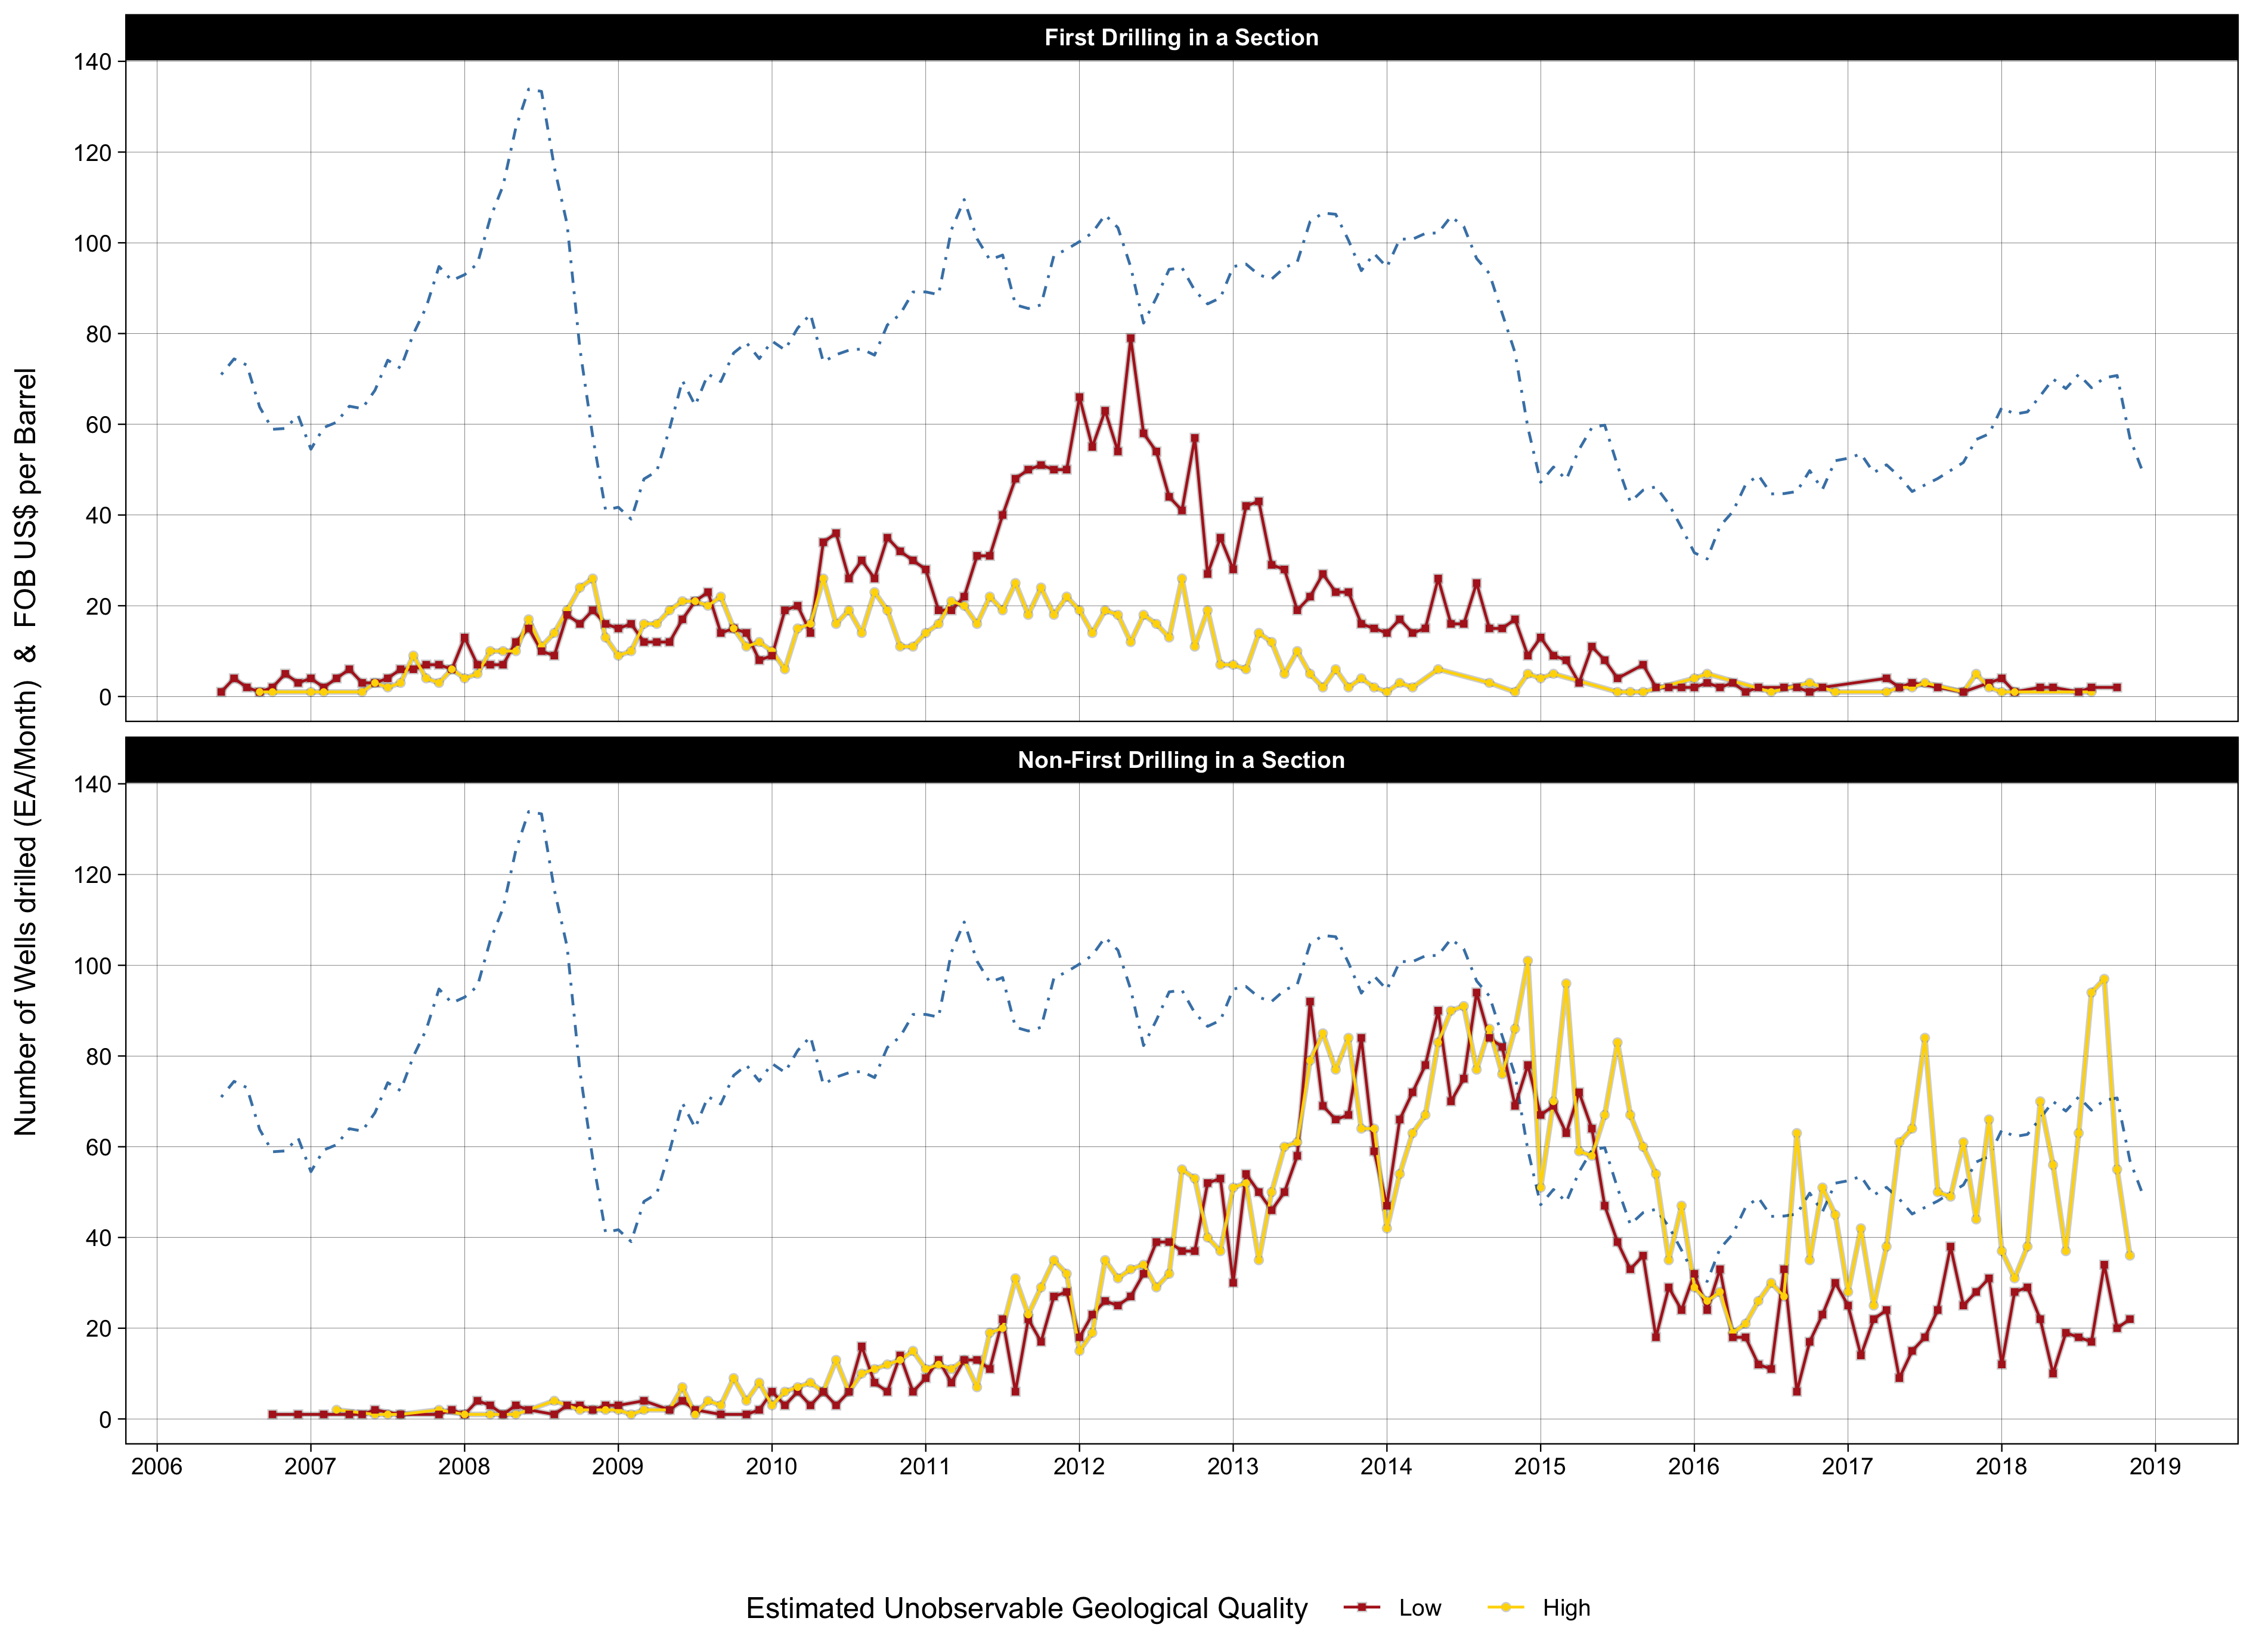
\includegraphics[scale = 0.12]{04_Chapter-3/00A_Figures/Figure_Drilling-over-Time_By-Well-Quality-and-Whether-First-Drilled.png}
        \caption{Held-by-Production vs. Non-Held-by-Production Horizontal Well Drilling}
        \caption*{
            {\small
            \textit{Note}: 
            This figure depicts the drilling of horizontal wells classified into two quality levels. The upper panel shows how the first drilling in each section, regarded as held-by-production drilling, has evolved. There was only a limited number of held-by-production drilling between 2015 and 2019. The lower panel indicates all subsequent drilling in sections. The collapse in oil prices between mid-2014 and 2015 made post-held-by-production drilling decrease. Drilling of low-quality well locations showed a more significant reduction, especially in 2015. High-quality sites were drilled more than low-quality ones during the period of oil price recovery from 2016 to 2019. In each panel, the dot-dashed line is the time series of the monthly per-barrel spot prices for West Texas Intermediate at Cushing, Oklahoma.
        }}
        \label{Figure:Held-by-Production-vs-Non-Held-by-Production-Horizontal-Well-Drilling}
    \end{figure}
}
Figure \ref{Figure:Held-by-Production-vs-Non-Held-by-Production-Horizontal-Well-Drilling} shows that drilling associated with held-by-production did not drive the relationship between oil prices and low-quality well drilling, especially between mid-2014 and the end of 2015. The upper panel in the figure illustrates the by-quality time series of the number of horizontal wells drilled that are supposed to be drilling related to Held-By-Production (HBP). In our empirical analysis, we assume that for each of the sections into which horizontal wells in our sample were drilled, the purpose of the first drilling in that section was just HBP.\footnote{In the Public Land Survey System, a \textit{section}, which is one of 36 sections in a township, is a one-mile-square area.} The relatively high drilling rate of low-quality wells, especially between mid-2011 and mid-2013, seems to be consistent with the empirical result of \cite{The-Economics-of-Time-Limited-Development-Options_2020_Herrnstadt-Kellogg-and-Lewis}: firms bound to a lease contract including use-it-or-lose-it requirements tend to drill low-productivity well locations just before the first lease expires.

The evolving pattern of drilling for each of the three quality levels presented in the lower panel of Figure \ref{Figure:Held-by-Production-vs-Non-Held-by-Production-Horizontal-Well-Drilling}, regarded as post-held-by-production drilling, shows completely different movements from those in the upper panel. Until 2014, horizontal wells of heterogeneous quality were drilled equally and at the same growth rate. But drilling of low-productivity horizontal wells more sensitively reacted to negative price shocks between mid-2014 and 2015, compared to drilling medium- and high-quality wells. The new theoretical approach, required to rationalize the simultaneous drilling of wells with heterogeneous qualities, needs to explain the high sensitivity of low-quality well drilling.
